\section{Graph Isomorphism Problem}

In Example \ref{exm:npc} we mentioned that Graph Isomorphism Problem is assumed to be neither $\P$ nor $\NPC$. For this reason it seems to belong to a special class and thus we will describe a DNA system which solves this very special problem. %!% vocitovat?

Following approach is very similar to 3-coloring if we consider $n$ colors instead. The problem can be stated: ``For a colorless graph $G$ and a graph $H$ where every vertex has different color, find a coloring of $G$ with all of those $n$ colors used exactly once $(1)$ such that these colored graphs are isomorphic $(2)$.'' Now one has to verify that:
\begin{enumerate}
	\item every ``color'' was used exactly once so that the coloring can define a bijection,
	\item edges and non-edges are preserved.
\end{enumerate}

If $k$ is odd, we add a separated vertex to both graphs resulting in $G'$ and $H'$. Then $G'$ is isomorphic with $H'$ if and only if $G$ is isomorphic with $H$. See example in Figure \ref{fig:graph_iso}.

\subsection*{Set of tiles}

\begin{description}
	\item[Bottom tiles.] These tiles have almost the same rules as in graph 3-coloring, the difference is that {\em all} single-color combinations can be omitted. $\frac{n}{2} \cdot n(n-1) \sim \frac{n^3}{2}$ tile types were required.
	\item[Bottom corner tiles.] These tiles are exactly the same like for $k$-clique. $2$ tile types were required.
	\item[Inner tiles.] These tiles are similar to those in graph $3$-coloring -- they are responsible for numerical ordering. The difference is which do exist and which do not. Firstly, there exist only tiles with different numbers and different colors. Now let us assume a tile with numbers $k$ and $l$ with colors $a$ and $b$, respectively. Note that numbers $k$ and $l$ correspond with vertices in graph $G$ and colors $a$ and $b$ correspond with vertices in graph $H$. This tile must verify the isomorphism property -- existence or non-existence of edge between appropriate vertices. Thus the tile exists if and only if
	$$\bigl(\{k,\,l\} \in E(G) \wedge \{a,\,b\} \in E(H)\bigr) \vee \bigl(\{k,\,l\} \notin E(G) \wedge \{a,\,b\} \notin E(H)\bigr) . $$
	For similar reasons all pairs of vertices from graph $G$ meet each other, thus every edge is verified so the condition $(2)$ is satisfied. Moreover it is verified that every color appears exactly once -- condition $(1)$: if a color appeared twice with different numbers, these numbers would meet each other and the tiling would stop because a tile with single-color combination does not exist. $4e^2 + 4\bigl(\binom{n}{2}-e\bigr)^2 + 2n(n-1) \sim 8e^2 - 4en^2 + n^4$ tile types were required.
	\item[Border tiles.] These tiles are exactly the same like for $k$-clique. $2$ tile types were required.
	\item[Verification tiles.] These tiles are almost the same like for graph $3$-coloring, the only difference is that there is a different number of color--number combinations. $n^2$ tile types were required.
	\item[DONE tile.] The tile is exactly the same like for $k$-clique. $1$ tile type was required.
\end{description}

Summed up, tile complexity of this DNA algorithm is asymptotically equivalent to $8e^2 - 4en^2 + n^4$. Binding complexity is asymptotically equivalent to $\nicefrac{5}{4}\,n^2$, glue complexity is asymptotically equivalent to $n^2$.

\begin{figure}[H]
\begin{center}
	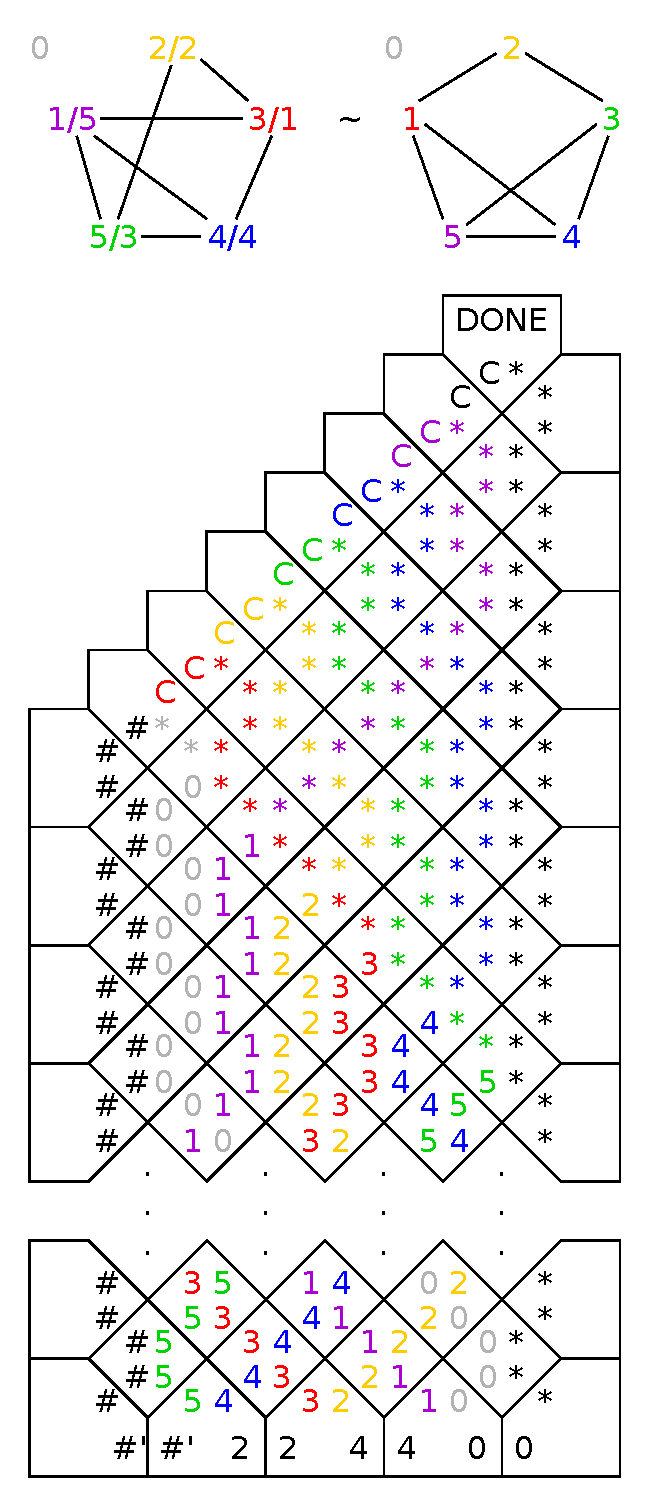
\includegraphics[scale=0.75]{./figures/isomorphism/isomorphism.pdf}
	\caption{Graph isomorphism computation. Color order is defined by their wavelength.}
	\label{fig:graph_iso}
\end{center}
\end{figure}
